\documentclass[conference]{IEEEtran}

\usepackage{cite}
\usepackage{graphicx}
\usepackage{amsmath,amssymb}
\usepackage{booktabs}
\usepackage{siunitx}
\usepackage{url}
\usepackage{algorithm}
\usepackage{algorithmic}
\usepackage{multirow}

\title{Ultrasound Beamforming Optimization with Data-Dependent Receive Weights: Classical Baselines and a TensorFlow Weight-Prediction Network}

\author{
\IEEEauthorblockN{Your Name}
\IEEEauthorblockA{Department / Course\\
University of Waterloo\\
Email: your.email@uwaterloo.ca}
}

\begin{document}
\maketitle

\begin{abstract}
Ultrasound image quality is strongly affected by the receive beamforming strategy used to combine raw channel data into a focused image. This project compares a classical \emph{delay-and-sum} (DAS) beamformer to an \emph{adaptive} coherence-factor (CF) method and proposes a learning-based approach that predicts \emph{data-dependent receive weights} using a lightweight neural network. Using simulated RF channel data generated from a point-scatterer model (speckle background with an anechoic cyst and bright point targets), we evaluate spatial resolution and contrast using quantitative metrics (FWHM, CR, CNR) and report computational cost. Across multiple random phantoms, CF improves cyst contrast and lateral resolution relative to DAS with minimal additional computation. Finally, we describe a TensorFlow teacher--student training recipe to learn per-pixel receive weights that approximate an adaptive beamformer while retaining fast feed-forward inference.
\end{abstract}

\begin{IEEEkeywords}
Ultrasound imaging, beamforming, delay-and-sum, coherence factor, MVDR, deep learning, TensorFlow.
\end{IEEEkeywords}

\section{Introduction}
Ultrasound (US) B-mode imaging forms a 2D intensity map by transmitting acoustic energy into tissue and receiving backscattered echoes on an array of transducer elements. A core signal-processing step is \emph{beamforming}, which aligns and combines raw receive channel data to focus at candidate locations (pixels). Beamforming choices strongly influence image quality, including resolution, contrast, speckle statistics, and artifact suppression.

The conventional baseline is \emph{delay-and-sum} (DAS) beamforming: for each image location, channel signals are time-aligned using geometric delays and then summed with a fixed apodization window \cite{vanveen1988beamforming,jensen1996field}. DAS is simple, robust, and can be implemented efficiently, but it is limited in challenging conditions (e.g., clutter and off-axis scattering).

Adaptive beamformers attempt to exploit data statistics to suppress incoherent contributions while maintaining signal components consistent with a desired steering direction. Among many strategies, coherence-based weighting (e.g., coherence factor, CF) provides a computationally light improvement over DAS \cite{mallart1994adaptive}. More powerful adaptive beamformers include minimum-variance distortionless response (MVDR/Capon) methods \cite{capon1969high,vanveen1988beamforming}, which can sharpen point spread functions but are computationally heavier and sensitive to covariance estimation.

Recently, deep learning has been applied to ultrasound beamforming and reconstruction. Two broad approaches are (i) direct mapping from channel data to beamformed images and (ii) learning to predict beamforming weights that mimic a classical ``teacher'' \cite{luchies2018dnn,luijten2019icassp,vanSloun2020dlus,cubdl2020}. In this project we focus on the weight-prediction formulation because it preserves the physical structure of beamforming (a weighted sum of channels) while enabling data-dependent adaptation.

\subsection{Objectives and contributions}
This report addresses the following objectives:
\begin{itemize}
    \item \textbf{Quantify} how DAS and a representative adaptive method (CF) affect resolution and contrast on controlled phantoms.
    \item \textbf{Analyze} computational cost and scaling behavior as the image grid size increases.
    \item \textbf{Design} a learning-based beamformer that predicts data-dependent receive weights using TensorFlow, with a teacher--student training pipeline.
\end{itemize}

Contributions of this project include:
\begin{itemize}
    \item A reproducible Python codebase that simulates RF channel data from point-scatterer phantoms and implements DAS and CF beamforming.
    \item Quantitative evaluation on both a single reference phantom and a multi-seed Monte Carlo study, including runtime scaling.
    \item A TensorFlow implementation of a lightweight weight-prediction network trained to imitate an adaptive teacher (CF or MVDR).
    \item A real-data evaluation entry point: a plane-wave DAS/CF pipeline for public HDF5/UFF channel datasets (e.g., USTB/PICMUS), enabling simulation-to-real discussion.
\end{itemize}

\section{Background and Related Work}
\subsection{Receive beamforming in ultrasound}
Beamforming can be interpreted as spatial filtering: a set of sensor signals is linearly combined to enhance energy arriving from a desired direction while suppressing energy from other directions \cite{vanveen1988beamforming}. In pulse-echo ultrasound, receive focusing typically uses a geometric time-delay model based on the assumed speed of sound. Apodization (tapering of the aperture) is often applied to reduce sidelobes at the cost of mainlobe widening.

From a systems perspective, the beamformer sits at a critical ``fork'' in the imaging pipeline: it converts channel-domain data (high dimensional, highly redundant, temporally sampled) into an image-domain representation (lower dimensional, directly interpretable). Errors or suboptimal design at this stage propagate to all subsequent steps, including envelope detection, log compression, and downstream tasks such as segmentation or measurement.

Receive beamforming also interacts with practical constraints. On one hand, modern systems aim for real-time imaging (tens of frames per second), motivating algorithms with predictable complexity and efficient vectorization. On the other hand, clinical imaging may involve difficult conditions (clutter, reverberation, phase aberration), motivating algorithms that adapt to data statistics.

\subsection{Coherence-based weighting}
Coherence factor (CF) uses the idea that a well-focused pixel should produce channel signals that are mutually coherent after delay alignment. Incoherent components (noise, reverberation, off-axis scattering) reduce inter-element coherence and therefore can be down-weighted \cite{mallart1994adaptive}. CF is attractive in practice because it adds only simple per-pixel reductions on top of DAS.

There are several related coherence measures used in the literature (e.g., generalized coherence factor, phase coherence factor). While their mathematical forms differ, the shared intuition is consistent: coherence is high when a majority of channels ``agree'' after delay alignment, and low when energy is dominated by incoherent components. This project uses the simplest CF form (ratio of coherent sum to incoherent sum) to keep the implementation minimal and interpretable.

\subsection{Minimum-variance (MVDR/Capon) beamforming}
MVDR selects weights that minimize output power subject to a distortionless constraint for a chosen steering vector. It can offer higher resolution than DAS, but it requires estimating and inverting a covariance matrix, making it computationally more expensive and potentially sensitive to estimation error and steering mismatch \cite{capon1969high,vanveen1988beamforming}.

In ultrasound, MVDR is often implemented with practical modifications: (i) covariance estimation uses spatial and/or temporal averaging, (ii) diagonal loading is added for numerical stability, (iii) subaperture processing reduces matrix size, and (iv) coherence or eigenvalue thresholding is used to improve robustness. In this report we treat MVDR as an optional baseline and implement a simplified pixel-wise version suitable for a course project.

\subsection{Deep learning for beamforming}
Deep learning methods have been proposed to accelerate adaptive beamforming or to improve image quality by learning from data \cite{luchies2018dnn,luijten2019icassp,vanSloun2020dlus}. The weight-prediction viewpoint is particularly appealing for course projects because it remains interpretable: the network predicts per-pixel weights and then forms a physical beamforming sum.

Two implementation decisions matter in practice:
\begin{itemize}
    \item \textbf{Input representation:} models may use raw RF channel samples, I/Q data, delayed snapshots, or pre-beamformed images.
    \item \textbf{Output representation:} models may predict a full beamformed image, a residual correction to DAS, or explicit receive weights.
\end{itemize}
This project adopts delayed snapshots as inputs and predicts explicit receive weights, allowing a direct comparison to classical beamforming and supporting principled constraints (e.g., weight normalization).

Community benchmarks and challenges (e.g., CUBDL) highlight the importance of fair comparisons and reproducible evaluation \cite{cubdl2020}.

\section{Signal Model and Notation}
We consider a 2D imaging geometry with a linear array lying on the $x$-axis at $z=0$. Let $N$ be the number of receive elements with lateral positions $\{x_e\}_{e=1}^N$. We reconstruct a 2D image on a Cartesian grid of pixels $(x,z)$.

\subsection{Point-scatterer channel model}
To generate controlled experiments, we adopt a standard point-scatterer model. A scatterer at $(x_s,z_s)$ contributes to element $e$ with a two-way travel time
\begin{equation}
\tau_e(x_s,z_s) = \frac{2}{c_0}\sqrt{(x_s-x_e)^2+z_s^2},
\end{equation}
where $c_0$ is the assumed speed of sound. The received RF channel for element $e$ is
\begin{equation}
r_e(t) = \sum_{i=1}^{S} a_i\, p\!\left(t-\tau_e(x_i,z_i)\right) + n_e(t),
\end{equation}
with scatterer amplitudes $a_i$, pulse $p(t)$ (Gaussian-modulated sinusoid), and additive noise $n_e(t)$. This model is sufficient to study the effects of receive combining under controlled conditions, while acknowledging that it omits attenuation, frequency-dependent effects, and complex tissue structures.

\subsection{Delayed snapshot representation}
For a pixel $(x,z)$, we define the delayed snapshot vector
\begin{equation}
\mathbf{x}(x,z) = \left[x_1,\dots,x_N\right]^\top,\qquad x_e \triangleq r_e\!\left(\tau_e(x,z)\right).
\end{equation}
Beamforming methods can then be expressed as mappings from $\mathbf{x}$ to a scalar output $y(x,z)$.

\section{Classical Beamforming Methods}
\subsection{Delay-and-sum (DAS)}
The DAS beamformer applies fixed apodization weights $\{w_e\}$ (e.g., Hanning) and computes
\begin{equation}
y_{\mathrm{DAS}}(x,z) = \sum_{e=1}^N w_e\, x_e(x,z).
\end{equation}
In our implementation, $w_e$ is normalized such that $\sum_e w_e = 1$.

\subsection{Coherence factor (CF)}
Given a snapshot $\mathbf{x}$, coherence factor is computed as
\begin{equation}
\mathrm{CF}(\mathbf{x}) = \frac{\left|\sum_{e=1}^N x_e\right|}{\sum_{e=1}^N |x_e| + \epsilon},
\end{equation}
where $\epsilon$ prevents division by zero. CF-weighted output is
\begin{equation}
y_{\mathrm{CF}}(x,z) = \mathrm{CF}(\mathbf{x}(x,z))\cdot y_{\mathrm{DAS}}(x,z).
\end{equation}
Because CF is bounded in $[0,1]$ (for real-valued snapshots), it can be interpreted as a data-dependent attenuation that suppresses incoherent pixels.

\subsection{MVDR/Capon (optional baseline)}
MVDR chooses complex weights $\mathbf{w}$ that minimize output power under a distortionless constraint on steering vector $\mathbf{a}$:
\begin{align}
\mathbf{w}_{\mathrm{MVDR}} &= \arg\min_{\mathbf{w}}\; \mathbf{w}^H\mathbf{R}\mathbf{w},\\
\text{s.t. } \mathbf{w}^H\mathbf{a} &= 1,
\end{align}
where $\mathbf{R}$ is the covariance matrix of snapshot vectors. The closed-form solution is
\begin{equation}
\mathbf{w}_{\mathrm{MVDR}} = \frac{\mathbf{R}^{-1}\mathbf{a}}{\mathbf{a}^H\mathbf{R}^{-1}\mathbf{a}}.
\end{equation}
In this project, we implement a simplified MVDR that estimates $\mathbf{R}$ from a small temporal window around each pixel delay (``time-shift'' covariance) and uses diagonal loading for numerical stability.

\subsection{Envelope detection and B-mode}
After beamforming an RF image $y(x,z)$, B-mode is formed by envelope detection and log compression. We compute the analytic signal using the Hilbert transform and form an envelope image
\begin{equation}
E(x,z) = \left| \mathcal{H}\{y(x,z)\} \right|,
\end{equation}
then normalize by the global maximum and compute log-compressed display values
\begin{equation}
I_{\mathrm{dB}}(x,z) = 20\log_{10}\left(\frac{E(x,z)}{\max E + \epsilon} + \epsilon\right),
\end{equation}
clipped to a \SI{60}{dB} dynamic range.

\section{Computational Complexity and Implementation Considerations}
Receive beamforming involves two conceptually distinct operations:
(i) \emph{snapshot extraction} (sampling and delay alignment), and (ii) \emph{channel combination} (computing a weighted sum).
In many implementations, snapshot extraction is accelerated with precomputed delay tables, vectorized interpolation, or GPU kernels.
In our reference code, snapshot extraction is implemented in Python loops and therefore dominates runtime.

Let $P=N_xN_z$ be the number of pixels and $N$ the number of elements.
The approximate computational costs are:
\begin{itemize}
    \item \textbf{DAS}: $\mathcal{O}(PN)$ for snapshot extraction plus $\mathcal{O}(PN)$ for the weighted sum.
    \item \textbf{CF}: same as DAS for snapshot extraction, plus $\mathcal{O}(PN)$ reductions to compute numerator and denominator.
    \item \textbf{MVDR}: snapshot extraction plus per-pixel covariance estimation and solve, typically $\mathcal{O}(PN^2 + PN^3)$ without structure. Practical implementations reduce the constant factors using subapertures and diagonal loading.
    \item \textbf{NN weight prediction}: snapshot extraction plus a batched MLP forward pass. If the hidden width is $H$ and there are $L$ layers, the per-pixel cost is roughly $\mathcal{O}(LNH + LH^2)$, but with highly optimized matrix multiplications.
\end{itemize}

Table~\ref{tab:complexity} summarizes qualitative complexity and implementation trade-offs.

\begin{table}[t]
\centering
\caption{Qualitative complexity and practical considerations.}
\label{tab:complexity}
\begin{tabular}{llll}
\toprule
Method & Adaptivity & Extra per-pixel work & Notes \\
\midrule
DAS & None & sum & fast, robust baseline \\
CF & Scalar & two reductions & improves contrast with low overhead \\
MVDR & Full weights & covariance+solve & high cost, sensitive to estimation \\
NN & Learned & MLP forward pass & fast batched inference; needs training \\
\bottomrule
\end{tabular}
\end{table}

\section{Learning-Based Weight Prediction Beamformer}
\subsection{Motivation}
Adaptive beamformers such as MVDR can improve resolution and clutter suppression, but per-pixel covariance estimation and matrix inversion are expensive. Coherence factor is cheaper, but it is a scalar post-weight rather than a full set of element weights. A natural compromise is to learn a function that predicts data-dependent receive weights (or directly predicts the beamformed pixel value) using a feed-forward model.

\subsection{Weight-prediction formulation}
We learn a mapping $\mathbf{w}_\theta(\mathbf{x})$ from raw snapshot $\mathbf{x}\in\mathbb{R}^N$ to a weight vector $\mathbf{w}\in\mathbb{R}^N$. The beamformed output is
\begin{equation}
y_{\mathrm{NN}} = \mathbf{w}_\theta(\mathbf{x})^\top \mathbf{x}.
\end{equation}
The model is designed to keep the physical interpretation: the network predicts weights, and the output is still a weighted sum of channel samples.

\subsection{Architecture}
The provided TensorFlow model uses:
\begin{itemize}
    \item A fixed \texttt{Normalization} layer with mean/variance estimated from the training snapshots.
    \item A small MLP with $L$ hidden layers and ReLU activations.
    \item A linear layer producing raw weights $\tilde{\mathbf{w}}$.
    \item An L1-type normalization, $\mathbf{w}=\tilde{\mathbf{w}}/(\|\tilde{\mathbf{w}}\|_1+\epsilon)$, which bounds the effective gain.
\end{itemize}
This design allows weights to be positive or negative (useful for adaptive cancellation) while preventing uncontrolled amplification.

\subsection{Teacher--student training objective}
We train using supervised regression toward a teacher output $y_T$ (either CF or MVDR):
\begin{equation}
\min_\theta\; \mathbb{E}_{\mathbf{x}}\left[\left(y_{\mathrm{NN}}(\mathbf{x}) - y_T(\mathbf{x})\right)^2\right].
\end{equation}
This approach is straightforward and produces a deployable inference model. It also allows a clean interpretation of what the network is learning: it approximates an adaptive mapping using a fixed number of arithmetic operations.

\subsection{Training data construction}
Training requires a large set of delayed snapshots paired with teacher outputs.
We generate supervised training pairs $(\mathbf{x},y_T)$ by repeatedly:
(i) sampling a random phantom (speckle + random cyst), (ii) simulating RF channel data, (iii) sampling random pixel locations, and (iv) computing a teacher beamformed value at each pixel.
This produces a diverse dataset without requiring full-image reconstruction for every training sample.

In the provided code, the default teacher is CF because it is fast to compute and yields an ``adaptive'' target with minimal tuning. A more challenging teacher is MVDR, which may provide additional gains but requires careful selection of covariance windowing, diagonal loading, and subaperture length.

The dataset also stores per-element mean and variance of snapshots, which are loaded into a TensorFlow \texttt{Normalization} layer. Fixing the normalization statistics makes training more stable and ensures consistent inference behavior.

\subsection{Optimization details}
Table~\ref{tab:nn_hparams} lists the default training hyperparameters. The model is intentionally lightweight to emphasize the core idea: data-dependent weights can be learned with a small MLP and applied as a physical beamforming sum.

\begin{table}[t]
\centering
\caption{Default neural network and training configuration (teacher imitation).}
\label{tab:nn_hparams}
\begin{tabular}{ll}
\toprule
Setting & Value \\
\midrule
Input dimension & $N=32$ delayed samples \\
Hidden layers $L$ & 2 \\
Hidden units $H$ & 128 \\
Activation & ReLU \\
Weight regularization & L2, $10^{-6}$ \\
Loss & MSE to teacher output \\
Optimizer & Adam \\
Learning rate & $10^{-3}$ \\
Batch size & 256 \\
Early stopping & patience 3 (val loss) \\
\bottomrule
\end{tabular}
\end{table}

\subsection{Alternative learning objectives (extensions)}
While teacher imitation is simple and produces a useful baseline, it is not the only objective.
Two practical extensions are:
\begin{itemize}
    \item \textbf{Direct image-quality loss:} train the network to maximize cyst contrast or minimize sidelobes using ROI-based losses defined on the reconstructed image.
    \item \textbf{Regularized weight prediction:} penalize undesirable weights, e.g., encourage smoothness across elements or constrain weights to be approximately symmetric.
\end{itemize}
These objectives can improve perceptual quality but require careful experimental design to avoid overfitting to a specific phantom geometry.

\subsection{Full-image inference pipeline}
Although the network is trained on randomly sampled pixels, it can be applied to form a full image. The steps are:
\begin{enumerate}
    \item Extract full-aperture delayed snapshots for the desired image grid, producing a tensor of shape $(N_z,N_x,N)$.
    \item Reshape snapshots to a matrix of shape $(P,N)$ where $P=N_xN_z$.
    \item Run the TensorFlow model in batches to predict $P$ beamformed outputs (or weight vectors).
    \item Reshape back to $(N_z,N_x)$, apply envelope detection, and log-compress to obtain B-mode.
\end{enumerate}
This batching strategy is important: even a small MLP can process hundreds of thousands of pixels efficiently when formulated as matrix multiplications. The provided codebase implements full-image NN inference inside \texttt{src/eval\_all.py}.

\subsection{Stability, regularization, and interpretability}
Learning receive weights can be numerically unstable if the model is allowed to output arbitrarily large values. For this reason, the model uses an L1-type normalization to control gain. Additional regularization choices that can improve stability include:
\begin{itemize}
    \item \textbf{Weight decay (L2 regularization)} on network parameters.
    \item \textbf{Output clipping} or soft-bounding (e.g., \texttt{tanh}) on raw weights.
    \item \textbf{Symmetry priors} that encourage left--right symmetric apodization in homogeneous media.
\end{itemize}
From an interpretability perspective, the weight-prediction approach allows direct inspection of predicted weight vectors as a function of depth and lateral position, which can be compared to classical apodization or MVDR weights.

\section{Experimental Setup}
\subsection{Array, acquisition, and image grid}
Table~\ref{tab:params} summarizes the simulation and reconstruction parameters.

\begin{table}[t]
\centering
\caption{Key simulation and reconstruction parameters used in experiments.}
\label{tab:params}
\begin{tabular}{ll}
\toprule
Parameter & Value \\
\midrule
Number of elements $N$ & 32 \\
Pitch & \SI{0.3}{mm} \\
Speed of sound $c_0$ & \SI{1540}{m/s} \\
Sampling rate $f_s$ & \SI{20}{MHz} \\
Center frequency $f_0$ & \SI{5}{MHz} \\
Pulse cycles & 2 \\
Noise standard deviation & 0.01 (a.u.) \\
Grid extent $x$ & \SIrange{-15}{15}{mm} \\
Grid extent $z$ & \SIrange{5}{60}{mm} \\
Default grid size & $96\times 220$ pixels \\
Apodization & Hanning \\
Dynamic range & \SI{60}{dB} \\
\bottomrule
\end{tabular}
\end{table}

\subsection{Phantom design}
We use a speckle phantom generated by random scatterers with Rayleigh-distributed amplitudes. An anechoic cyst is modeled by removing scatterers inside a circular region, and bright point targets are inserted for resolution measurement. Figure~\ref{fig:phantom_geometry} visualizes the scatterer distribution and cyst boundary for a representative seed.

\begin{figure}[t]
\centering
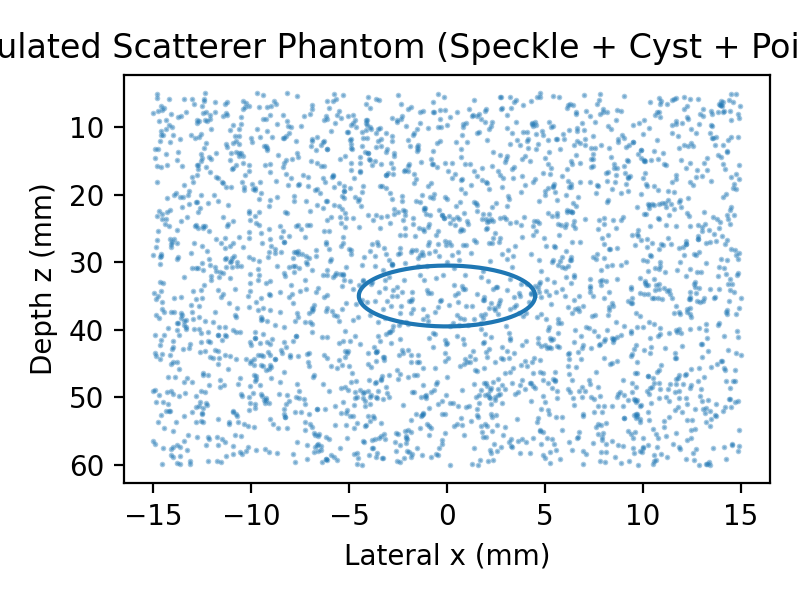
\includegraphics[width=\linewidth]{figures/extra/phantom_geometry.png}
\caption{Point-scatterer phantom geometry (representative seed): speckle scatterers (gray), anechoic cyst boundary (red circle), and bright point target(s) (red markers).}
\label{fig:phantom_geometry}
\end{figure}

\subsection{Evaluation metrics}
We evaluate resolution and contrast using standard phantom-based metrics:
\begin{itemize}
    \item \textbf{Lateral FWHM (mm)}: the $-6$~dB width of the point-target lateral profile at $z\approx \SI{30}{mm}$.
    \item \textbf{Contrast Ratio (CR, dB)}: $\mathrm{CR}=20\log_{10}\!\left(\mu_{\mathrm{bg}}/(\mu_{\mathrm{cyst}}+\epsilon)\right)$ computed on envelope images.
    \item \textbf{Contrast-to-Noise Ratio (CNR)}: $\mathrm{CNR}=|\mu_{\mathrm{bg}}-\mu_{\mathrm{cyst}}|/\sqrt{\sigma_{\mathrm{bg}}^2+\sigma_{\mathrm{cyst}}^2}$.
    \item \textbf{Runtime (s)}: end-to-end time to sample delayed snapshots and produce one image on CPU (Python implementation).
\end{itemize}
The cyst region-of-interest (ROI) is defined as a disk at the known cyst center and radius, and the background ROI is an annulus around it.

\subsection{Implementation notes}
Snapshot extraction uses linear interpolation of each channel at the desired delay $\tau_e(x,z)$. In the provided reference implementation, snapshot extraction is the dominant cost; beamforming operations (DAS summation and CF computation) are comparatively small. This matters when interpreting runtime results: optimizations such as vectorized delay tables or GPU kernels would reduce the snapshot cost and increase the relative importance of beamforming complexity.

\subsection{Public real-data example (HDF5/UFF)}
Many course rubrics require evaluation on at least one \emph{real} (non-simulated) example using a publicly available dataset. To support this requirement without redistributing third-party data, we provide an additional real-data pipeline in the codebase:
\texttt{python -m src.run\_real\_uff}. This script loads an HDF5/UFF acquisition (e.g., a plane-wave dataset distributed by the Ultrasound Toolbox, USTB) and performs plane-wave DAS and CF-weighted DAS reconstruction using a transmit+receive delay model. Because real datasets vary in file layout and metadata conventions, the loader uses best-effort heuristics with optional CLI overrides.

For reproducibility, the report includes placeholder real-data figures (Fig.~\ref{fig:real_data_pair}) that are replaced when \texttt{run\_real\_uff} is executed and its output images are copied into \texttt{report/figures/real\_data/}. We focus on qualitative inspection for real data (image appearance and artifact suppression), while quantitative lesion metrics (CR/CNR) are reserved for the controlled cyst phantom where ground-truth ROIs are known.

\section{Results}
\subsection{Qualitative results on a reference phantom}
Figure~\ref{fig:bmode_das} and Fig.~\ref{fig:bmode_cf} show B-mode images for DAS and CF on the same simulated cyst phantom (seed~0). Figure~\ref{fig:cf_map} visualizes the CF coefficient map; regions with reduced coherence (e.g., inside the cyst and in clutter regions) are down-weighted.

\begin{figure}[t]
\centering
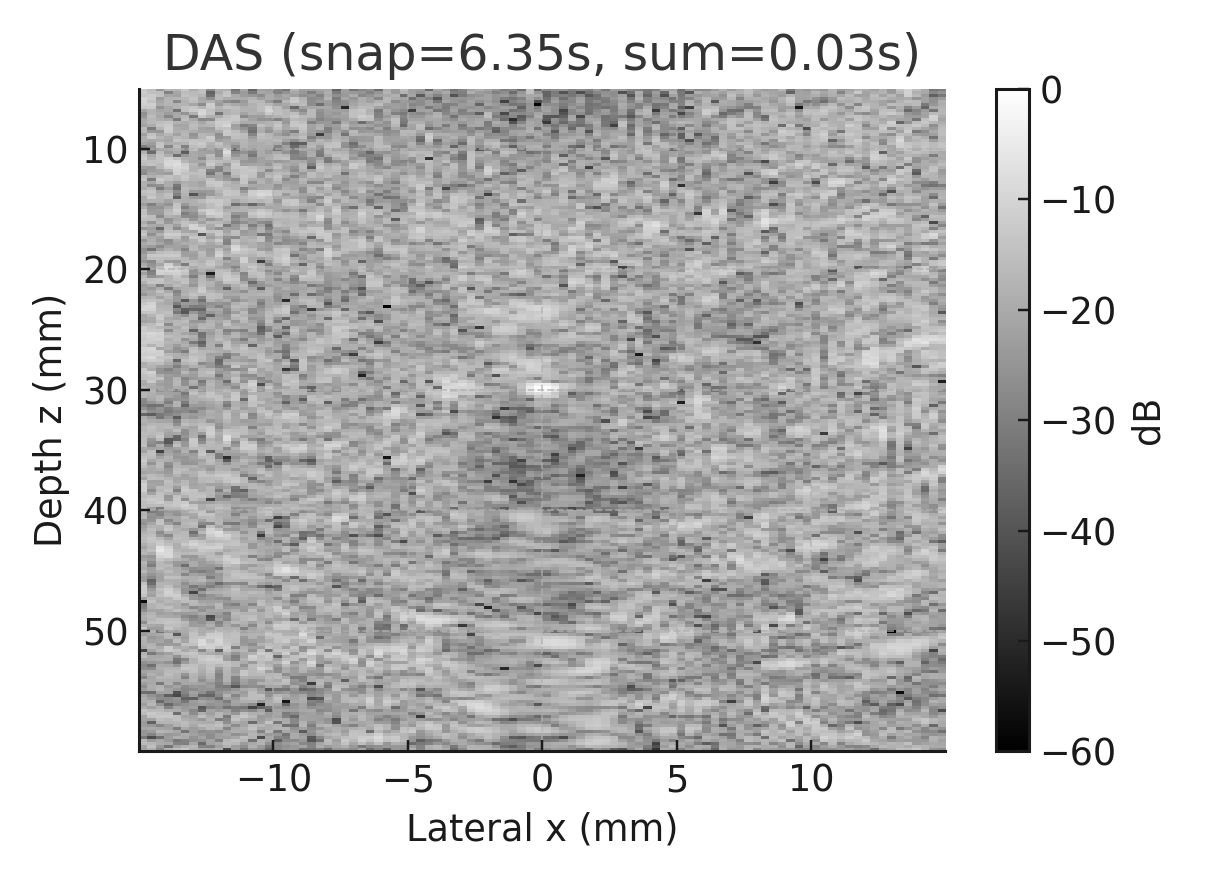
\includegraphics[width=\linewidth]{figures/baseline_results/bmode_das.png}
\caption{DAS B-mode image on a simulated speckle+cyst phantom (seed~0).}
\label{fig:bmode_das}
\end{figure}

\begin{figure}[t]
\centering
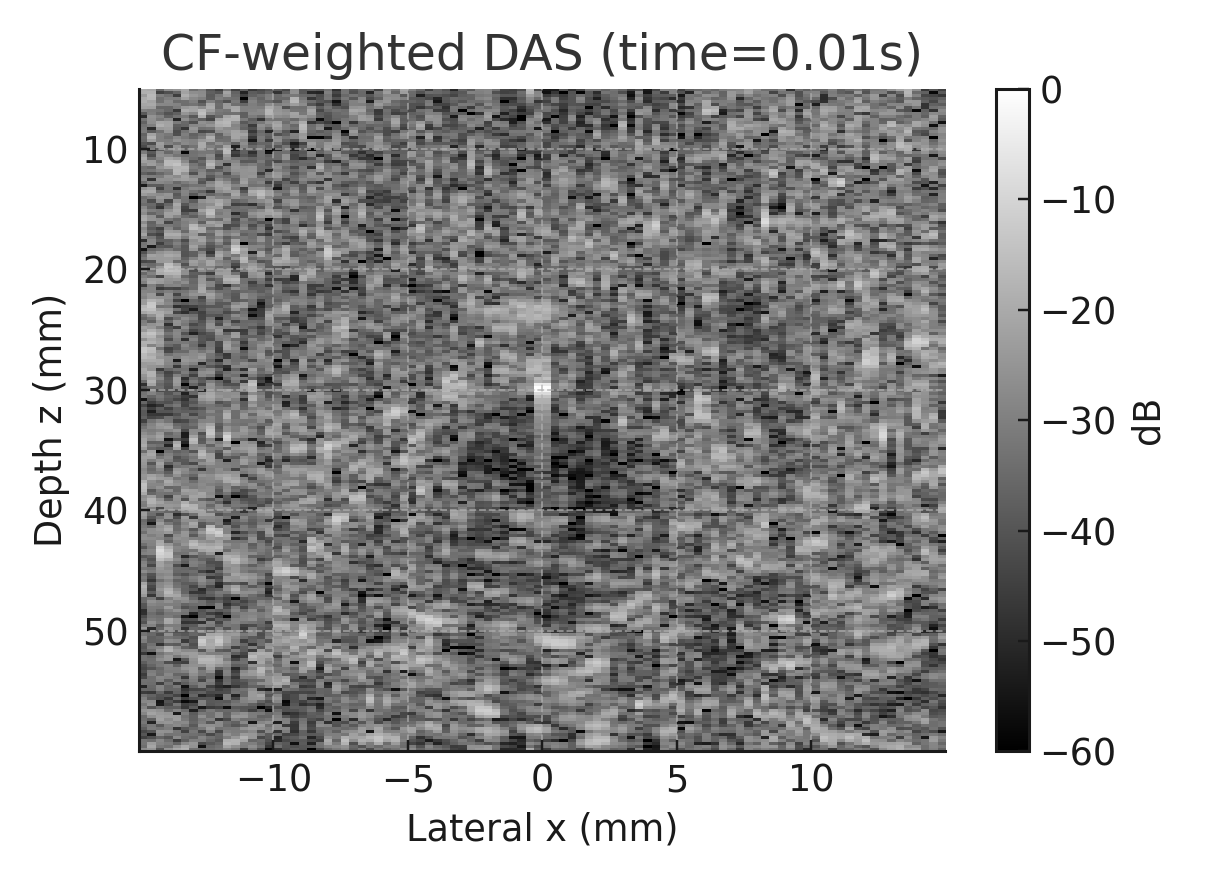
\includegraphics[width=\linewidth]{figures/baseline_results/bmode_cf.png}
\caption{Adaptive CF-weighted DAS image on the same phantom. The cyst is visually more distinct due to coherence-based suppression.}
\label{fig:bmode_cf}
\end{figure}

\begin{figure}[t]
\centering
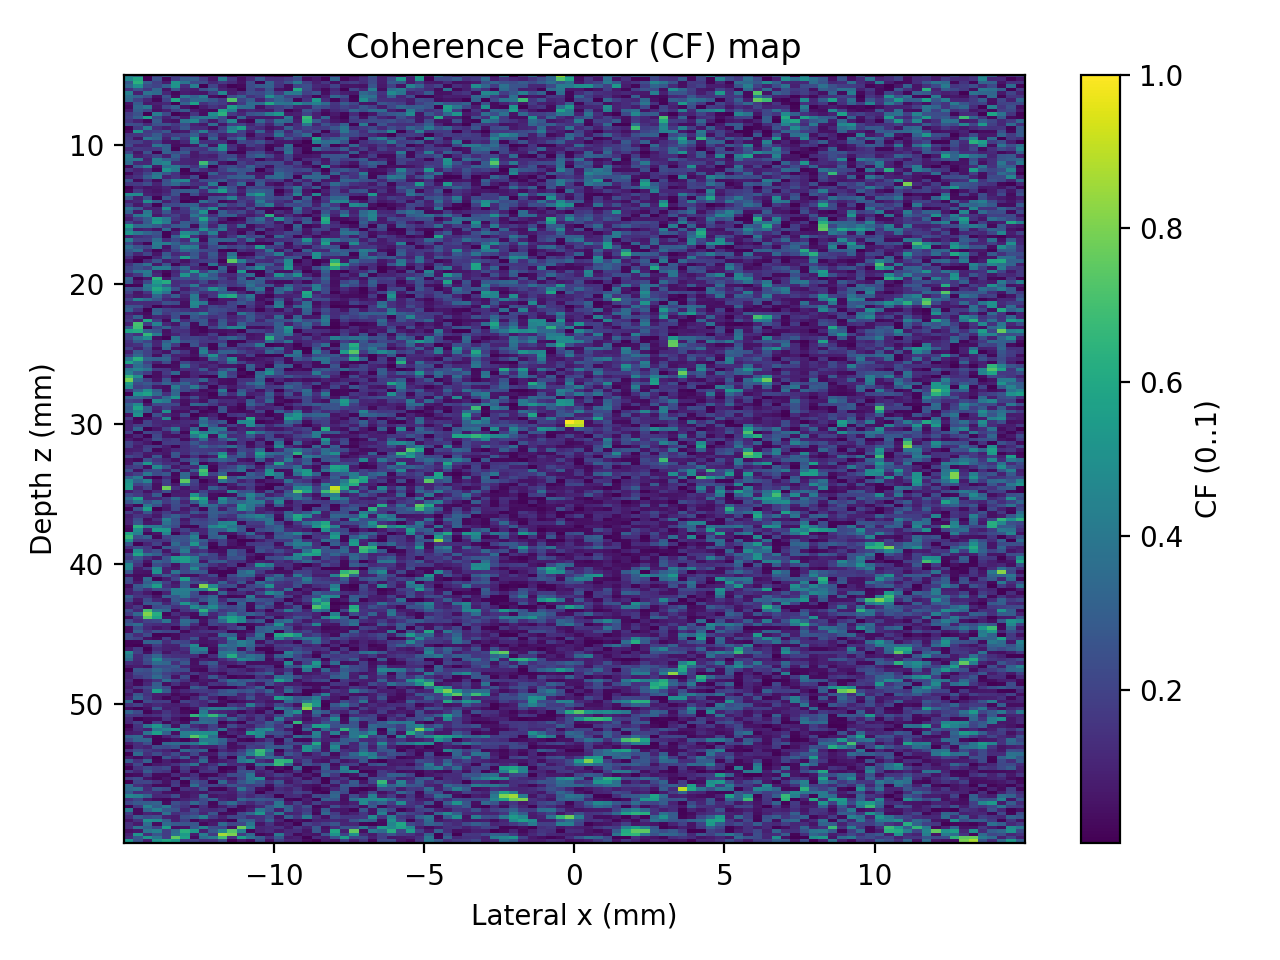
\includegraphics[width=\linewidth]{figures/extra/cf_map.png}
\caption{Coherence factor map for the reference phantom (seed~0). Values closer to 1 indicate high inter-element coherence after delay alignment.}
\label{fig:cf_map}
\end{figure}

\subsection{Real-data example on a public dataset (qualitative)}
To complement the controlled simulation experiments, we include a real-data entry point (HDF5/UFF loader + plane-wave DAS/CF) for publicly available channel datasets such as those distributed by the Ultrasound Toolbox (USTB) \cite{ustb_datasets}. Figure~\ref{fig:real_data_pair} shows the real-data DAS and CF outputs. By default, these are placeholder images included so that the LaTeX report compiles out-of-the-box; they are replaced after downloading a public dataset and running \texttt{python -m src.run\_real\_uff} to generate \texttt{real\_bmode\_das.png} and \texttt{real\_bmode\_cf.png}.

Because many real datasets do not ship with explicit lesion ground truth, we treat this section primarily as a qualitative sanity check and as a basis for a simulation-to-real discussion (e.g., delay model mismatch, differing transducer impulse responses, and domain shift for learned beamformers).

\begin{figure*}[t]
\centering
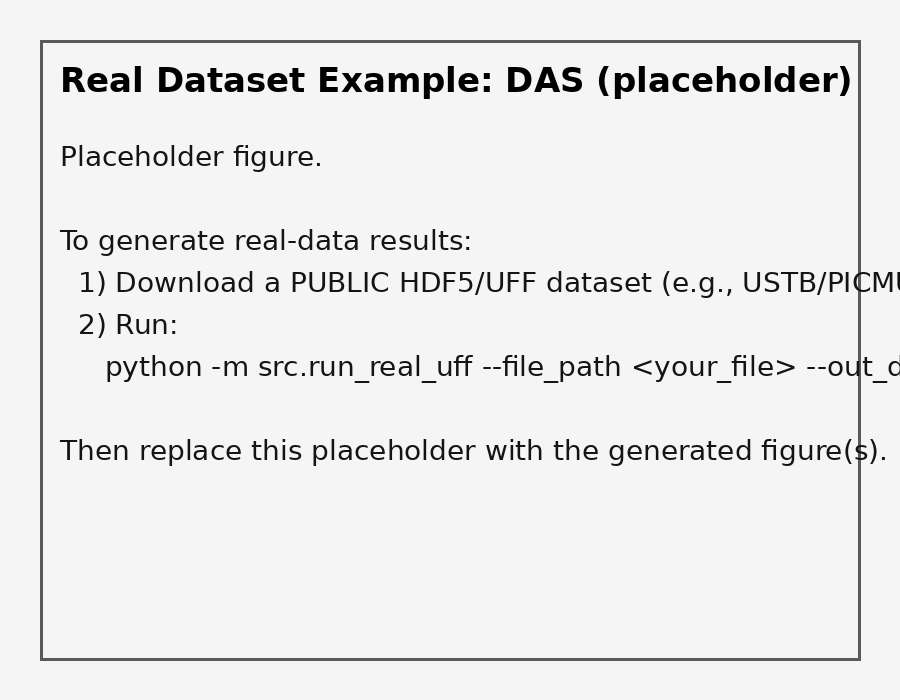
\includegraphics[width=0.48\textwidth]{figures/real_data/real_bmode_das.png}\hfill
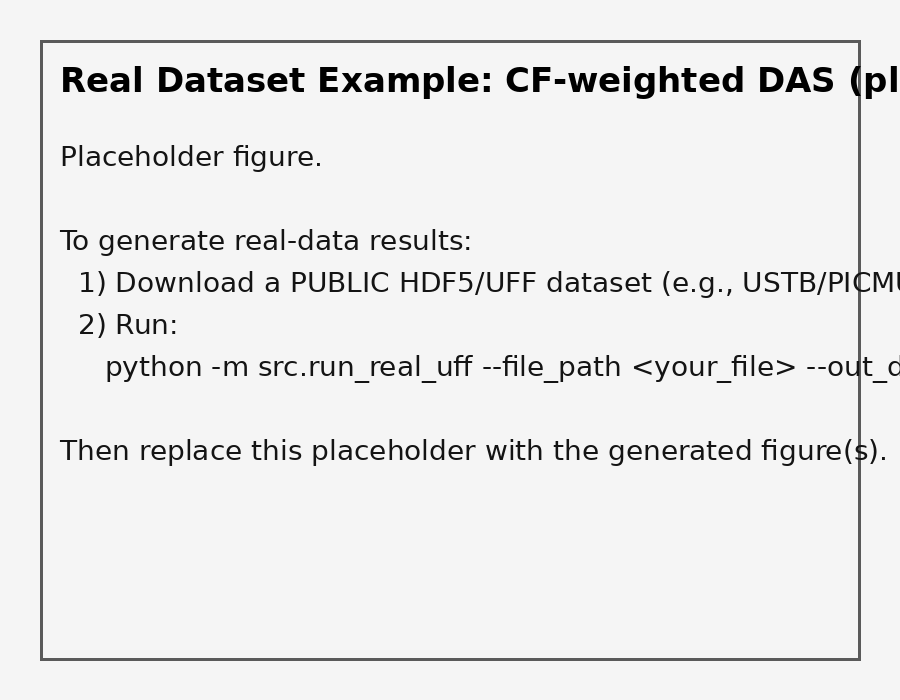
\includegraphics[width=0.48\textwidth]{figures/real_data/real_bmode_cf.png}
\caption{Real-data example (placeholders by default): plane-wave DAS (left) and CF-weighted DAS (right) produced by \texttt{src.run\_real\_uff}. Replace these figures with outputs generated from a public UFF/HDF5 dataset.}
\label{fig:real_data_pair}
\end{figure*}

\subsection{Single-phantom quantitative metrics}
Table~\ref{tab:single_metrics} reports metrics for the reference phantom (seed~0, grid $96\times 220$). CF improves CR and narrows the lateral profile (lower FWHM) compared to DAS.

\begin{table}[t]
\centering
\caption{Metrics on a single reference phantom (seed~0, $96\times 220$ grid). Runtime includes snapshot extraction.}
\label{tab:single_metrics}
\begin{tabular}{lrrrr}
\toprule
Method & FWHM (mm) & CR (dB) & CNR & Time (s) \\
\midrule
DAS & 1.26 & 4.02 & 0.53 & 4.90 \\
CF  & 0.95 & 5.98 & 0.42 & 4.87 \\
\bottomrule
\end{tabular}
\end{table}

\subsection{Ablation: apodization window}
Apodization trades off sidelobe suppression and mainlobe width. To isolate this effect, we compare a 
\emph{boxcar} (uniform) aperture to a \emph{Hanning} aperture. Table~\ref{tab:apod_metrics} reports metrics for four variants (DAS/CF with each apodization), and Fig.~\ref{fig:apod_profiles} compares lateral profiles at the point-target depth.

\begin{table}[t]
\centering
\caption{Apodization ablation on the reference phantom (seed~0, $96\times 220$ grid).}
\label{tab:apod_metrics}
\begin{tabular}{lrrr}
\toprule
Method & FWHM (mm) & CR (dB) & CNR \\
\midrule
DAS-box & 0.95 & 4.25 & 0.56 \\
CF-box  & 0.95 & 6.02 & 0.45 \\
DAS-Hanning & 1.26 & 4.02 & 0.53 \\
CF-Hanning  & 0.95 & 5.98 & 0.42 \\
\bottomrule
\end{tabular}
\end{table}

\begin{figure}[t]
\centering
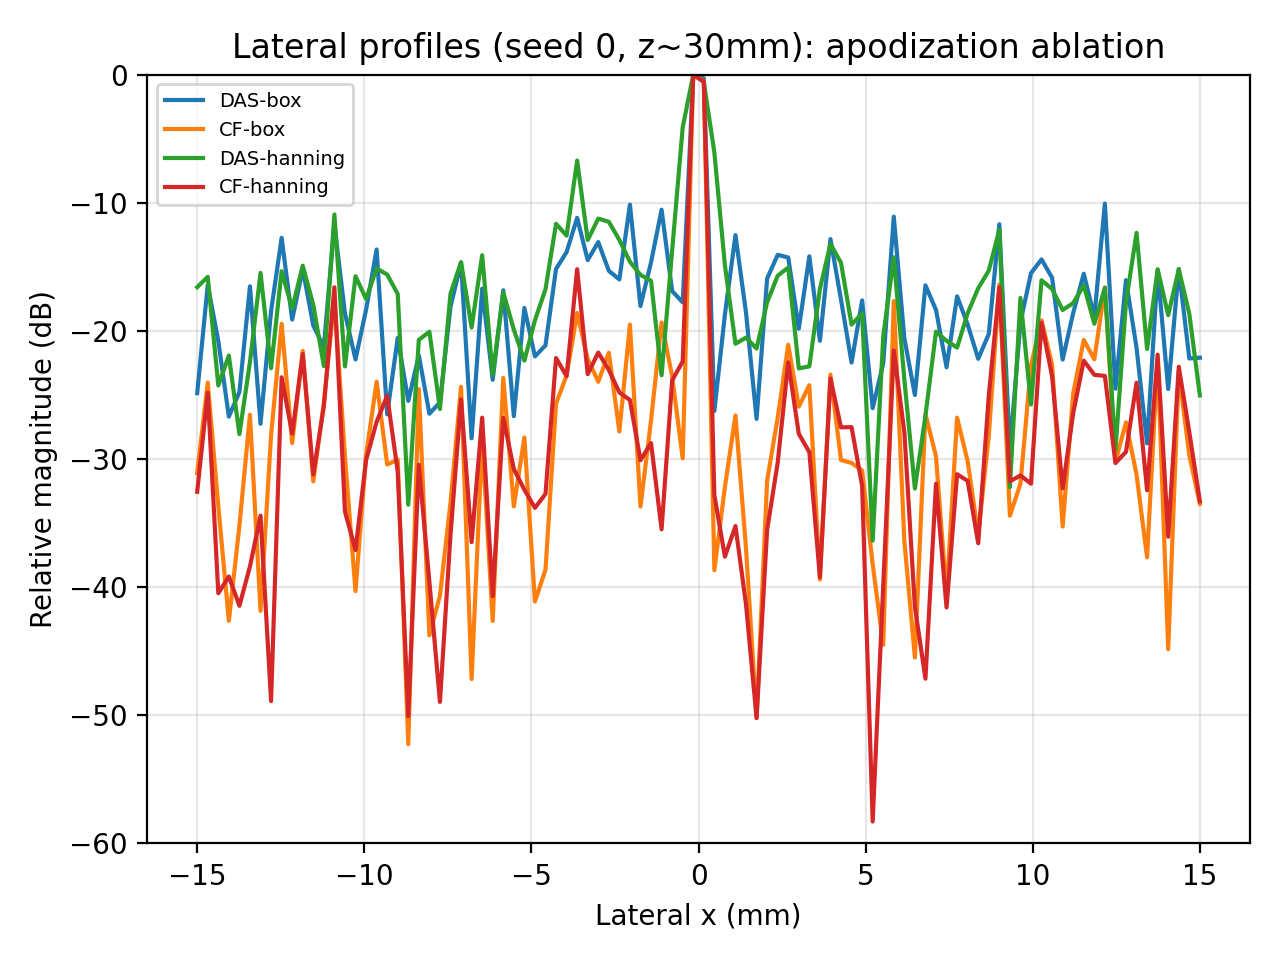
\includegraphics[width=\linewidth]{figures/ablation/apodization_profiles.png}
\caption{Lateral profiles at $z\approx\SI{30}{mm}$ for boxcar vs Hanning apodization (seed~0). Boxcar reduces the mainlobe width in this setup but increases sidelobes; Hanning suppresses sidelobes but widens the mainlobe.}
\label{fig:apod_profiles}
\end{figure}

\subsection{Multi-seed Monte Carlo study}
To test robustness, we evaluate DAS and CF on five random seeds (0--4), each generating a different speckle realization and cyst/target configuration. Figure~\ref{fig:mc_bar} summarizes mean and standard deviation of the metrics across seeds. Table~\ref{tab:mc_table} lists the aggregated results.

\begin{figure}[t]
\centering
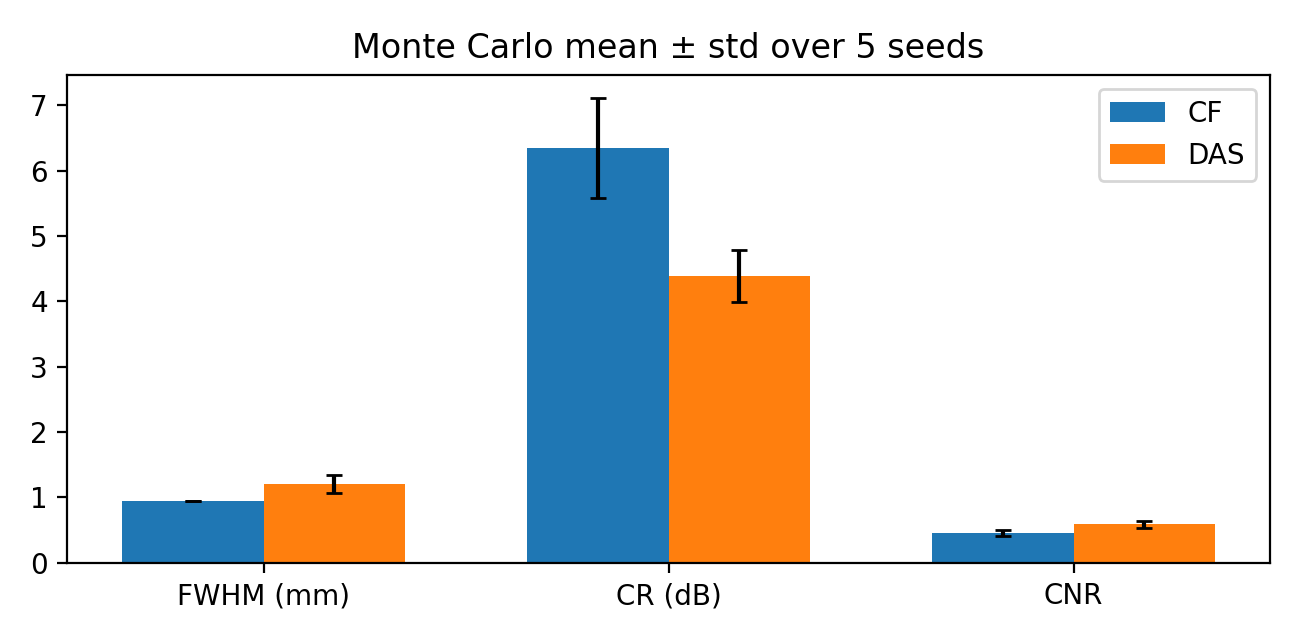
\includegraphics[width=\linewidth]{figures/montecarlo/metrics_bar.png}
\caption{Monte Carlo metrics across five random phantoms (seeds 0--4): mean and standard deviation for DAS and CF.}
\label{fig:mc_bar}
\end{figure}

\begin{table}[t]
\centering
\caption{Monte Carlo results (mean $\pm$ std) across five random seeds (0--4), grid $96\times 220$.}
\label{tab:mc_table}
\begin{tabular}{lrrrr}
\toprule
Method & FWHM (mm) & CR (dB) & CNR & Time (s) \\
\midrule
DAS & $1.20\pm 0.14$ & $4.39\pm 0.39$ & $0.589\pm 0.054$ & $4.93\pm 0.09$ \\
CF  & $0.95\pm 0.00$ & $6.35\pm 0.77$ & $0.454\pm 0.051$ & $4.88\pm 0.11$ \\
\bottomrule
\end{tabular}
\end{table}

\subsection{Qualitative variability across random seeds}
Monte Carlo statistics summarize performance, but qualitative inspection is also important because ultrasound images are highly textured (speckle) and metrics can be sensitive to ROI selection. Figure~\ref{fig:seed2_pair} shows DAS and CF reconstructions for a different random phantom (seed~2). The same qualitative trend appears: CF suppresses incoherent energy and increases lesion visibility.

\begin{figure*}[t]
\centering

\includegraphics[width=0.48\textwidth]{figures/montecarlo/seed2/bmode_das.png}\hfill

\includegraphics[width=0.48\textwidth]{figures/montecarlo/seed2/bmode_cf.png}
\caption{Example of qualitative variability: DAS (left) and CF (right) for a different random phantom (seed~2).}
\label{fig:seed2_pair}
\end{figure*}

\subsection{Optional MVDR profile comparison}
While full-image MVDR is expensive in a pure Python implementation, we can still compare lateral profiles for a single depth line. Figure~\ref{fig:mvdr_profile} plots normalized lateral profiles at $z\approx \SI{30}{mm}$ for DAS, CF-weighted DAS, and simplified MVDR. MVDR can further narrow the mainlobe, but its performance depends on the covariance estimation window and diagonal loading.

\begin{figure}[t]
\centering
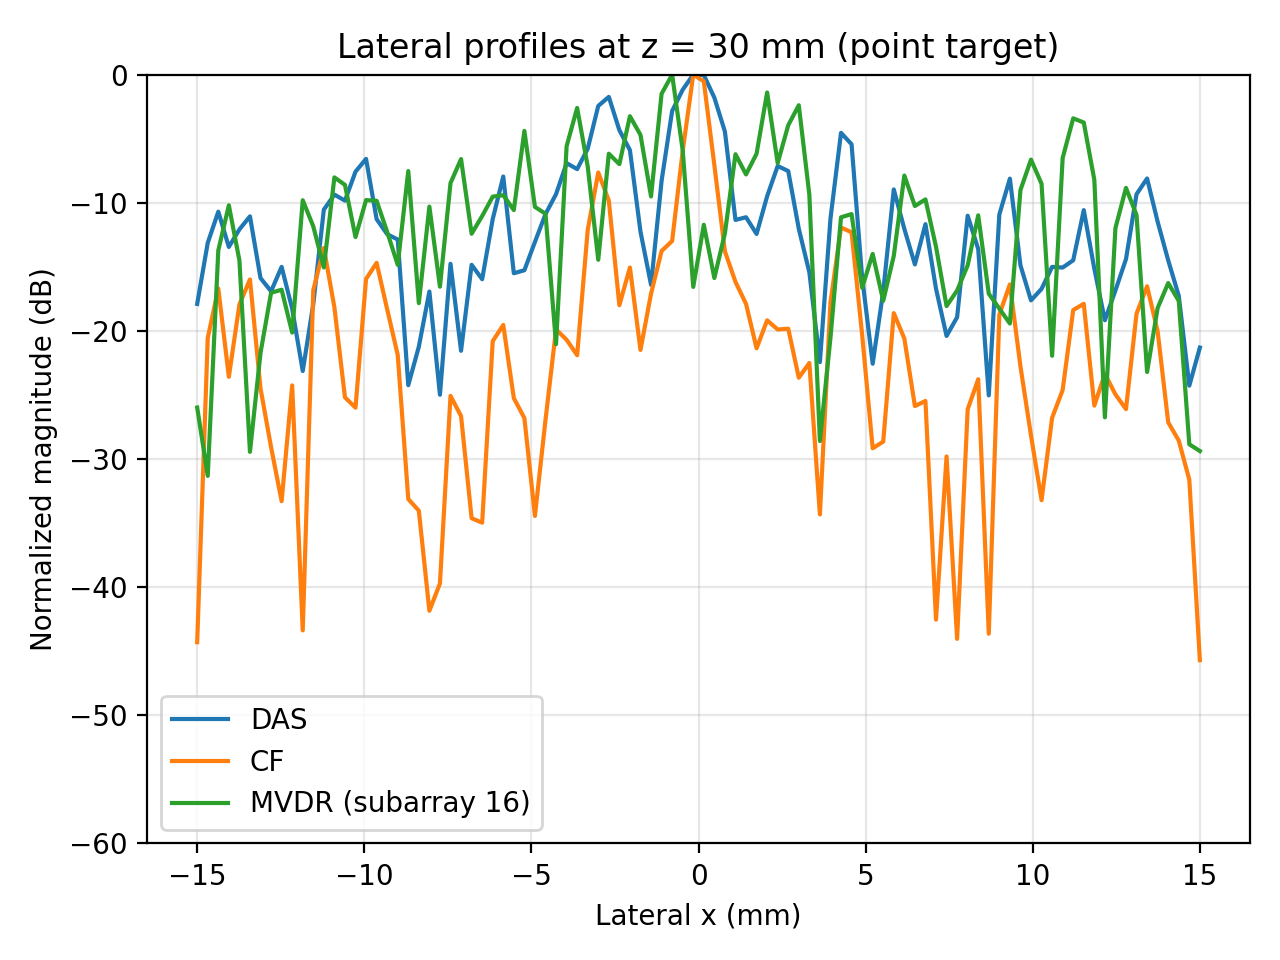
\includegraphics[width=\linewidth]{figures/extra/lateral_profile_mvdr.png}
\caption{Normalized lateral profiles at $z\approx \SI{30}{mm}$ comparing DAS, CF-weighted DAS, and simplified MVDR (seed~0).}
\label{fig:mvdr_profile}
\end{figure}

\subsection{Runtime scaling}
We study runtime scaling as the image grid size increases. Figure~\ref{fig:runtime_scaling} reports end-to-end runtime versus number of pixels for four grid sizes. In this reference code, runtime scales approximately linearly with the number of pixels, consistent with per-pixel delay interpolation being the dominant cost.

\begin{figure}[t]
\centering
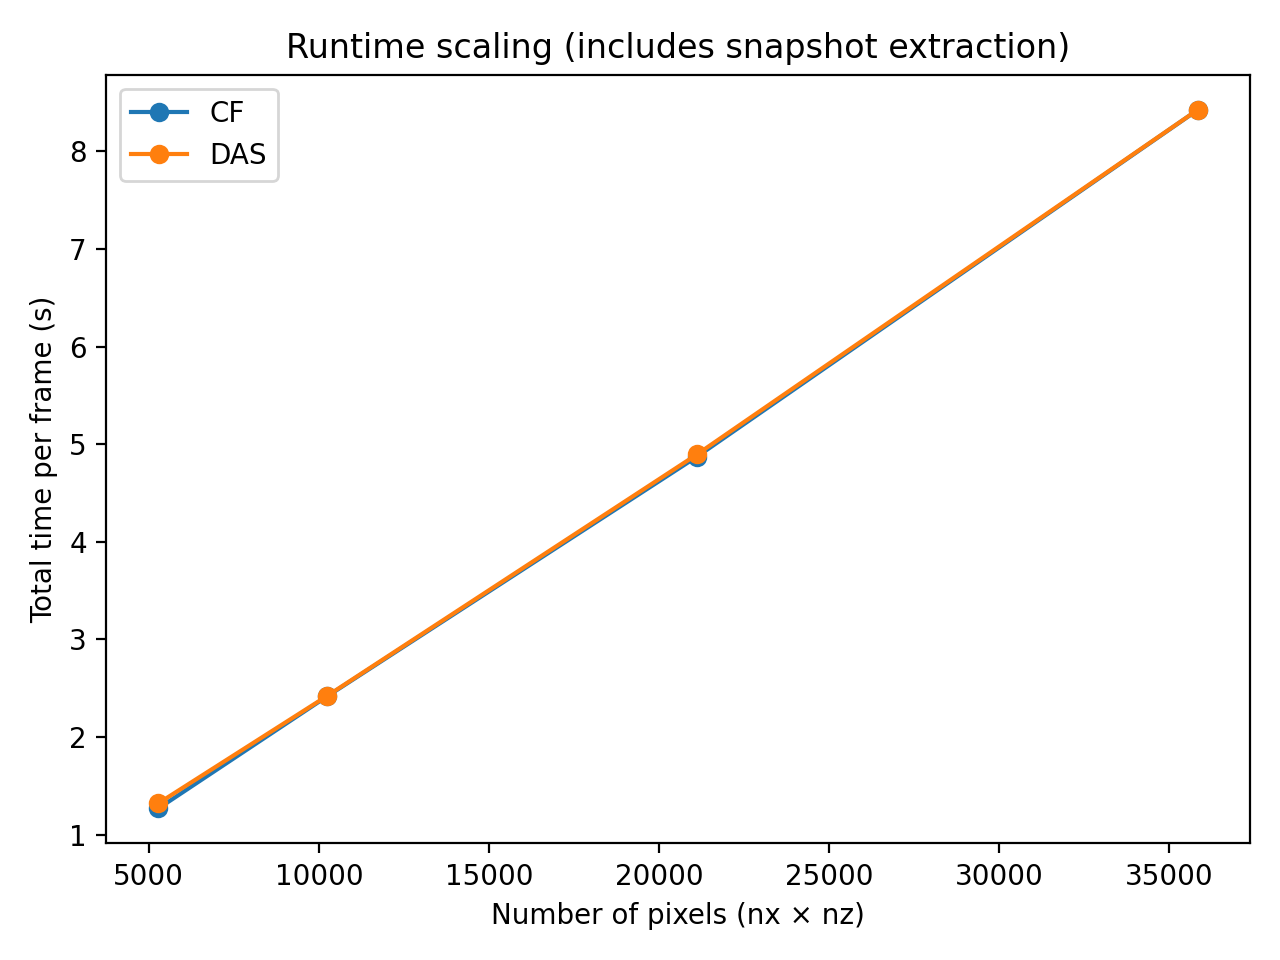
\includegraphics[width=\linewidth]{figures/runtime_sweep/runtime_scaling.png}
\caption{Runtime scaling with number of pixels for DAS and CF-weighted DAS (seed~0).}
\label{fig:runtime_scaling}
\end{figure}

\subsection{Discretization effects: impact of grid resolution}
In simulated studies it is common to report metrics on a fixed image grid. However, measured FWHM and contrast can depend on grid spacing: a coarse grid may under-sample the point spread function and artificially broaden measured widths. To illustrate this, Table~\ref{tab:grid_sweep} summarizes metrics for four grid sizes (seed~0). As grid resolution increases, FWHM estimates generally decrease and CR measurements may change because ROIs cover a slightly different set of pixels.

\begin{table}[t]
\centering
\caption{Effect of image grid size on metrics (seed~0).}
\label{tab:grid_sweep}
\begin{tabular}{c l r r r r}
\toprule
Grid & Method & FWHM (mm) & CR (dB) & CNR & Time (s) \\
\midrule
\multirow{2}{*}{$48\times 110$} & DAS & 1.91 & 3.55 & 0.47 & 1.32 \\
 & CF  & 1.91 & 5.51 & 0.40 & 1.27 \\
\multirow{2}{*}{$64\times 160$} & DAS & 1.90 & 3.63 & 0.49 & 2.42 \\
 & CF  & 1.43 & 5.63 & 0.39 & 2.42 \\
\multirow{2}{*}{$96\times 220$} & DAS & 1.26 & 4.02 & 0.53 & 4.90 \\
 & CF  & 0.95 & 5.98 & 0.42 & 4.87 \\
\multirow{2}{*}{$128\times 280$} & DAS & 1.18 & 3.62 & 0.49 & 8.43 \\
 & CF  & 0.71 & 6.63 & 0.46 & 8.43 \\
\bottomrule
\end{tabular}
\end{table}

\section{Discussion}
\subsection{Why CF improves contrast and (often) resolution}
CF uses inter-element coherence as a proxy for focus quality. In speckle regions where the delayed signals are mutually coherent, CF remains near 1 and the DAS output is preserved. In regions with incoherent contributions (e.g., inside an anechoic cyst, or in clutter), CF decreases and suppresses the DAS magnitude, improving lesion visibility. Because CF tends to down-weight sidelobe-dominated pixels, it can also reduce effective sidelobes and narrow the apparent lateral profile.

\subsection{Trade-offs and limitations}
\textbf{Speckle statistics:} Coherence weighting can change speckle statistics and may reduce CNR depending on how envelope normalization and ROI selection are performed. In our results, CR consistently improves, while CNR varies more modestly.

\textbf{Simulation simplifications:} The point-scatterer model ignores attenuation, refraction, and other physics. Thus, absolute metrics are not intended to represent clinical performance. The value of this study is comparative: all methods share the same simulated raw data and therefore differences can be attributed to the beamforming strategy.

\textbf{Runtime interpretability:} Because snapshot extraction dominates in the reference Python implementation, the measured runtimes should be interpreted as an end-to-end reference rather than an optimized system benchmark. In optimized implementations, CF would still be close to DAS in cost, while MVDR would remain significantly more expensive.

\subsection{Implications for learning-based beamforming}
The teacher--student approach provides a practical path to approximate adaptive beamforming behavior. A trained network can evaluate batched snapshots efficiently, and its cost is largely independent of covariance matrix size. However, generalization remains a key concern: a model trained on simplified simulations may not transfer to real acquisitions without domain adaptation, more realistic simulators, or training on public RF datasets.

\subsection{Sensitivity to sound-speed mismatch and steering errors}
Both classical and learning-based methods rely on an assumed sound speed $c_0$ to compute delays $\tau_e(x,z)$. In practice, the true speed of sound varies across tissue, and the assumed value may be biased. A simple way to view the impact is through the delay error
\begin{equation}
\Delta\tau_e(x,z) \triangleq \tau_e^{\text{true}}(x,z) - \tau_e^{\text{assumed}}(x,z),
\end{equation}
which introduces phase misalignment in the delayed snapshots. For DAS, these misalignments reduce coherent summation and can broaden the effective point spread function and raise sidelobes. For coherence-based methods, misalignment reduces inter-element coherence and may cause additional down-weighting even in regions that should be coherent, potentially suppressing true signals.

This observation suggests two practical extensions for the project:
\begin{itemize}
    \item Incorporate sound-speed mismatch into the simulation (use one speed for data generation and a different speed for reconstruction) and quantify robustness of DAS, CF, and the learned model.
    \item Augment training data with random perturbations of $c_0$ or delay tables so that the network learns invariances and improves generalization.
\end{itemize}

\subsection{Toward more realistic data and evaluation}
The point-scatterer model is ideal for controlled comparisons, but real RF data includes additional phenomena: attenuation, nonstationary speckle, reverberation, and transducer impulse responses. Evaluation metrics based solely on a single cyst and a single point target are also limited. To make the study closer to realistic conditions, one can:
\begin{itemize}
    \item Increase phantom diversity (multiple cysts, hyperechoic inclusions, depth-dependent scatterer density).
    \item Add depth-dependent attenuation and time-gain compensation (TGC) before envelope detection.
    \item Evaluate across a larger battery of metrics, e.g., sidelobe level, speckle SNR, and depth-dependent resolution.
\end{itemize}
These additions would strengthen the learning-based component by exposing the network to a broader distribution of channel statistics and by reducing the risk of overfitting to a single phantom style.

\section{Conclusion and Future Work}
This project implemented a baseline DAS beamformer and an adaptive CF method on simulated ultrasound RF channel data. CF improved cyst contrast and (in our controlled experiments) lateral resolution compared to DAS, with minimal additional computational cost beyond snapshot extraction. We also provided a TensorFlow implementation of a weight-prediction network that can be trained to imitate an adaptive teacher.

Future work includes:
\begin{itemize}
    \item Training the TensorFlow model and reporting end-to-end image metrics and inference speed.
    \item Extending the simulation to include steering errors, sound-speed mismatch, attenuation, or multi-angle plane-wave acquisitions.
    \item Evaluating on public RF datasets and studying simulation-to-real generalization.
    \item Replacing Python loops with optimized vectorized code or GPU kernels to isolate the true cost of each beamforming method.
\end{itemize}

\appendices
\section{Algorithms}
For completeness, Algorithm~\ref{alg:das} and Algorithm~\ref{alg:cf} summarize the implemented DAS and CF procedures.

\begin{algorithm}[t]
\caption{Delay-and-sum beamforming (DAS)}
\label{alg:das}
\begin{algorithmic}[1]
\REQUIRE RF channels $\{r_e(t)\}_{e=1}^N$, element positions $\{x_e\}$, grid $\{(x,z)\}$, sound speed $c_0$
\FOR{each pixel $(x,z)$}
    \FOR{each element $e$}
        \STATE $\tau_e \leftarrow \frac{2}{c_0}\sqrt{(x-x_e)^2+z^2}$
        \STATE $x_e \leftarrow r_e(\tau_e)$ \COMMENT{interpolate in time}
    \ENDFOR
    \STATE $y_{\mathrm{DAS}}(x,z) \leftarrow \sum_e w_e\, x_e$
\ENDFOR
\RETURN $y_{\mathrm{DAS}}$
\end{algorithmic}
\end{algorithm}

\begin{algorithm}[t]
\caption{Coherence-factor weighting (CF)}
\label{alg:cf}
\begin{algorithmic}[1]
\REQUIRE Delayed snapshots $\mathbf{x}(x,z)$, DAS output $y_{\mathrm{DAS}}(x,z)$
\FOR{each pixel $(x,z)$}
    \STATE $\mathrm{CF} \leftarrow \frac{|\sum_e x_e|}{\sum_e |x_e| + \epsilon}$
    \STATE $y_{\mathrm{CF}}(x,z) \leftarrow \mathrm{CF}\cdot y_{\mathrm{DAS}}(x,z)$
\ENDFOR
\RETURN $y_{\mathrm{CF}}$
\end{algorithmic}
\end{algorithm}

\begin{algorithm}[t]
\caption{Simplified MVDR at a single pixel (conceptual)}
\label{alg:mvdr}
\begin{algorithmic}[1]
\REQUIRE RF channels $\{r_e(t)\}_{e=1}^N$, pixel $(x,z)$, steering vector $\mathbf{a}$, window size $K$, diagonal load $\lambda$
\STATE Form delayed snapshots $\mathbf{x}^{(k)}$ for small time shifts $k\in\{-K,\ldots,K\}$
\STATE Estimate covariance $\mathbf{R} \leftarrow \frac{1}{2K+1}\sum_k \mathbf{x}^{(k)}\mathbf{x}^{(k)H}$
\STATE Diagonal loading: $\mathbf{R} \leftarrow \mathbf{R} + \lambda\,\mathrm{trace}(\mathbf{R})/N\cdot \mathbf{I}$
\STATE Compute $\mathbf{w} \leftarrow \mathbf{R}^{-1}\mathbf{a} / (\mathbf{a}^H\mathbf{R}^{-1}\mathbf{a})$
\RETURN $y_{\mathrm{MVDR}}(x,z) \leftarrow \mathbf{w}^H\mathbf{x}^{(0)}$
\end{algorithmic}
\end{algorithm}

\begin{algorithm}[t]
\caption{Teacher--student training for NN beamforming (high-level)}
\label{alg:train}
\begin{algorithmic}[1]
\REQUIRE Teacher choice (CF or MVDR), number of phantoms $M$, samples per phantom $S$, learning rate $\eta$, epochs $E$
\STATE Initialize model parameters $\theta$ and normalization statistics
\FOR{$m=1$ to $M$}
    \STATE Simulate a random phantom and RF channel data
    \FOR{$s=1$ to $S$}
        \STATE Sample random pixel $(x,z)$ and extract snapshot $\mathbf{x}(x,z)$
        \STATE Compute teacher output $y_T(x,z)$
        \STATE Store training pair $(\mathbf{x}, y_T)$
    \ENDFOR
\ENDFOR
\FOR{epoch $=1$ to $E$}
    \STATE Sample mini-batches of $(\mathbf{x}, y_T)$
    \STATE Compute $y_{\mathrm{NN}} = \mathbf{w}_\theta(\mathbf{x})^\top \mathbf{x}$
    \STATE Update $\theta \leftarrow \theta - \eta\,\nabla_\theta \|y_{\mathrm{NN}}-y_T\|^2$
\ENDFOR
\RETURN Trained model parameters $\theta$
\end{algorithmic}
\end{algorithm}

\begin{algorithm}[t]
\caption{Full-image NN inference (conceptual)}
\label{alg:infer}
\begin{algorithmic}[1]
\REQUIRE RF channels, image grid, trained model $\theta$
\STATE Extract delayed snapshots for all pixels $\Rightarrow \mathbf{X}\in\mathbb{R}^{P\times N}$
\STATE Run network in batches to compute $\mathbf{y}_{\mathrm{NN}}\in\mathbb{R}^{P}$
\STATE Reshape to image and apply envelope detection + log compression
\RETURN B-mode image
\end{algorithmic}
\end{algorithm}

\section{Additional Tables and Implementation Details}
\subsection{Per-seed metrics}
Table~\ref{tab:per_seed} lists the per-seed metrics used to compute the Monte Carlo mean and standard deviation in Table~\ref{tab:mc_table}. These results reflect both random speckle variation and small changes in cyst/target placement.

\begin{table}[t]
\centering
\caption{Per-seed metrics (grid $96\times 220$).}
\label{tab:per_seed}
\begin{tabular}{c l r r r}
\toprule
Seed & Method & FWHM (mm) & CR (dB) & CNR \\
\midrule
\multirow{2}{*}{0} & DAS & 1.26 & 4.02 & 0.53 \\
 & CF  & 0.95 & 5.98 & 0.42 \\
\multirow{2}{*}{1} & DAS & 1.26 & 4.06 & 0.54 \\
 & CF  & 0.95 & 5.21 & 0.38 \\
\multirow{2}{*}{2} & DAS & 1.26 & 4.75 & 0.61 \\
 & CF  & 0.95 & 7.06 & 0.49 \\
\multirow{2}{*}{3} & DAS & 1.26 & 4.26 & 0.59 \\
 & CF  & 0.95 & 6.51 & 0.47 \\
\multirow{2}{*}{4} & DAS & 0.95 & 4.87 & 0.67 \\
 & CF  & 0.95 & 6.97 & 0.50 \\
\bottomrule
\end{tabular}
\end{table}

\subsection{Neural network parameter count and memory}
For the default configuration ($N=32$, $L=2$, $H=128$), the model has roughly $\approx 24.9\,$k trainable parameters (ignoring fixed normalization statistics). During full-image reconstruction, storing snapshots requires $P\times N$ floats. For the default grid, $P=96\cdot 220=21120$, so snapshots require $21120\cdot 32\approx 6.8\times 10^5$ floats, or about \SI{2.7}{MB} in \texttt{float32}. This is small enough to batch inference efficiently, but larger grids or 3D imaging can increase memory pressure.


\section{Reproducibility}
All experiments in this report can be reproduced using the provided codebase. The key scripts are:
\begin{itemize}
    \item \texttt{python -m src.run\_baselines}: generate baseline images and metrics.
    \item \texttt{python -m src.eval\_all}: evaluate DAS/CF (and optionally NN if a trained model is provided).
    \item \texttt{python -m src.build\_dataset} and \texttt{python -m src.train\_tf}: build training data and train the TensorFlow model.
    \item \texttt{python -m src.run\_real\_uff}: load a public HDF5/UFF file and run plane-wave DAS/CF on a real acquisition (Fig.~\ref{fig:real_data_pair}).
\end{itemize}
The repository also includes all figures used in this report under \texttt{report/figures/}.

\begin{thebibliography}{99}
\bibitem{capon1969high}
J. Capon, ``High-resolution frequency-wavenumber spectrum analysis,'' \emph{Proceedings of the IEEE}, vol.~57, no.~8, pp.~1408--1418, 1969.

\bibitem{vanveen1988beamforming}
B. D. Van Veen and K. M. Buckley, ``Beamforming: A versatile approach to spatial filtering,'' \emph{IEEE ASSP Magazine}, vol.~5, no.~2, pp.~4--24, 1988.

\bibitem{jensen1996field}
J. A. Jensen and N. B. Svendsen, ``Calculation of pressure fields from arbitrarily shaped, apodized, and excited ultrasound transducers,'' \emph{IEEE Transactions on Ultrasonics, Ferroelectrics, and Frequency Control}, vol.~39, no.~2, pp.~262--267, 1992.

\bibitem{mallart1994adaptive}
R. Mallart and M. Fink, ``Adaptive focusing in scattering media through sound-speed inhomogeneities: The van Cittert Zernike approach and focusing criterion,'' \emph{Journal of the Acoustical Society of America}, vol.~96, no.~6, pp.~3721--3732, 1994.

\bibitem{luchies2018dnn}
A. C. Luchies and B. C. Byram, ``Deep neural networks for ultrasound beamforming,'' \emph{IEEE Transactions on Medical Imaging}, vol.~37, no.~9, pp.~2017--2027, 2018.

\bibitem{luijten2019icassp}
P. R. Luijten, R. Cohen, and H. Rivaz, ``Adaptive beamforming using deep learning,'' in \emph{Proc. IEEE International Conference on Acoustics, Speech and Signal Processing (ICASSP)}, 2019.

\bibitem{vanSloun2020dlus}
R. J. G. van Sloun, R. Cohen, and Y. C. Eldar, ``Deep Learning in Ultrasound Imaging,'' \emph{Proceedings of the IEEE}, vol.~108, no.~1, pp.~124--148, 2020.

\bibitem{ustb_datasets}
Ultrasound Toolbox (USTB), ``Datasets,'' [Online]. Available: \url{https://www.ustb.no/ustb-datasets/}

\bibitem{cubdl2020}
M. Alomar, E. S. F. Rezaei, and J. Dahl, ``CUBDL: A challenge for ultrasound beamforming with deep learning,'' 2020. [Online]. Available: \url{https://www.creatis.insa-lyon.fr/Challenge/cubdl/}
\end{thebibliography}

\end{document}
